\documentclass[12pt]{article}
\usepackage[utf8]{inputenc}
\usepackage{enumerate}
\usepackage{amsmath}
\usepackage{amssymb}
\usepackage{graphicx}
\usepackage{amsfonts}
\usepackage{array}
\usepackage{hyperref}
\usepackage[margin=1.2in,footskip=0.25in]{geometry}
\usepackage{wrapfig}

\hypersetup{
    colorlinks=true,
    linkcolor=blue,
    filecolor=magenta,      
    urlcolor=blue,
    pdftitle={Overleaf Example},
    pdfpagemode=FullScreen,
    }
%matriz ampliada
\newcommand{\uvec}[1]{\boldsymbol{\hat{\textbf{#1}}}}

\makeatletter
\renewcommand*\env@matrix[1][*\c@MaxMatrixCols c]{%
  \hskip -\arraycolsep
  \let\@ifnextchar\new@ifnextchar
  \array{#1}}
\makeatother

\AtBeginEnvironment{pmatrix}{\setlength{\arraycolsep}{5pt}}

%! TEX root = "~/home/ramiro/main.tex"
\setlength{\parindent}{0pt}
\title{\Huge{Conceptos de Sistemas Operativos\\
Modulo 1}}
\author{\huge{Ramiro Cabral}}
\date{\huge{}}

\begin{document}
\maketitle
\tableofcontents
\pagebreak

\pagebreak

\section{Conceptos Básicos}
\begin{itemize}
    \item \textbf{Sistema Operativo:} Software que actúa como intermediario entre el usuario de una computadora y su hardware.
\end{itemize}

\subsection{Objetivos de un SO}
\begin{itemize}
    \item \textbf{Comodidad:} Hacer más fácil el uso del hardware.
    \item \textbf{Eficiencia:} Hacer un uso más eficiente de los recursos del sistema.
    \item \textbf{Evolución:} Permitirá la introducción de nuevas funciones al sistema sin interferir con funciones anteriores.
\end{itemize}

\subsection{Perspectiva desde el usuario}
\begin{itemize}
    \item Abstracción con respecto a la arquitectura.
    \item El SO "oculta" el hardware y presenta a los programas abstracciones más simples de manejar.
    \item Los programas de aplicación son los clientes del SO.
\end{itemize}

\subsection{Perspectiva desde la administración de recursos}
\begin{itemize}
    \item Administra los recursos de HW de uno o más procesos.
    \item Provee un conjunto de servicios a los usuarios del sistema.
    \item Maneja la memoria secundaria y los dispositivos de E/S.
    \item Ejecución simultánea de procesos.
    \item Multiplexión en tiempo (CPU) y en espacio (memoria).
\end{itemize}

\subsection{Componentes de un SO}
\begin{itemize}
    \item \textbf{Kernel}
    \item \textbf{Shell}
    \item \textbf{Herramientas}
\end{itemize}

\subsubsection{Kernel}
\begin{itemize}
    \item Porción de código que se encuentra en memoria principal y se encarga de la administración de los recursos.
    \item Implementa servicios esenciales:
        \begin{itemize}
            \item Manejo de la memoria y la entrada/salida.
            \item Manejo de la CPU.
            \item Administración de procesos.
        \end{itemize}
\end{itemize}

\subsection{Servicios de un SO}
\begin{itemize}
    \item Administración y planificación del procesador.
    \item Administración de la memoria.
    \item Administración del almacenamiento/sistema de archivos.
    \item Administración de dispositivos.
    \item Detección de errores y respuestas.
        \begin{itemize}
            \item Errores de HW internos y externos.
            \item Errores de SW.
            \item Incapacidad del SO para conceder una solicitud de una aplicación.
        \end{itemize}
    \item Interacción con el usuario (Shell).
    \item Telemetría.
\end{itemize}

\subsection{Errores que un SO debe evitar}
\begin{itemize}
    \item Que un proceso se apropie de la CPU.
    \item Que un proceso intente ejecutar instrucciones de E/S, por ejemplo.
    \item Que un proceso intente acceder a una dirección de memoria que no le corresponde.
\end{itemize}

\pagebreak

\section{Apoyo del Hardware}
\begin{itemize}
    \item Modos de Ejecución: Limitaciones en el conjunto de instrucciones que se pueden ejecutar en cada modo.
    \item Interrupción de Clock: Se debe evitar que un proceso se apropie de la CPU.
    \item Protección de la Memoria: Se deben definir límites de memoria a los que puede acceder cada proceso.
\end{itemize}

\subsection{Modos de Ejecución}
\begin{itemize}
    \item Un bit en la CPU indica el modo actual.
    \item Las instrucciones privilegiadas solo pueden ejecutarse en modo \textbf{supervisor/Kernel}.
    \item En modo \textbf{Usuario}, el proceso puede acceder solo a su espacio de direcciones, es decir, a las direcciones "propias".
    \item El kernel del SO se ejecuta en modo supervisor.
    \item El resto del SO y los programas de usuario se ejecutan en modo usuario.
\end{itemize}

\subsubsection{Modo Kernel}
\begin{itemize}
    \item \textbf{Gestión de procesos:} Creación y terminación, planificación, intercambio, sincronización y soporte para la comunicación entre procesos.
    \item \textbf{Gestión de memoria:} Reserva de espacio de direcciones para los procesos, Swapping, Gestión de Páginas.
    \item \textbf{Gestión E/S:} Gestión de buffers, reserva de canales de E/S y de dispositivos de los procesos.
    \item \textbf{Funciones de soporte:} Gestión de interrupciones, auditoría, monitoreo.
    \item Cada vez que comienza a ejecutarse un proceso de usuario, el bit de modo se debe poner en modo usuario.
    \item Cuando hay una trap, el bit de modo se pone en modo Kernel. Esta es la única forma de pasar a modo Kernel.
\end{itemize}

\subsubsection{Modo Usuario}
\begin{itemize}
    \item Debug de procesos, definición de protocolos de comunicación, gestión de aplicaciones.
    \item Tareas que no requieran accesos privilegiados.
    \item No se puede interactuar con el hardware.
    \item Cada proceso trabaja en su propio espacio de direcciones.
\end{itemize}

\subsection{Protección de la E/S}
\begin{itemize}
    \item Las instrucciones de E/S se definen como privilegiadas.
    \item Deben ejecutarse en Modo Kernel.
    \item Los procesos de usuario realizan E/S a través de System Calls.
\end{itemize}

\subsection{Protección de la CPU}
\begin{itemize}
    \item Uso de interrupción por clock para evitar que un proceso se apropie de la CPU.
    \item Las instrucciones que modifican el funcionamiento del reloj son privilegiadas.
\end{itemize}

\subsection{System Calls}
\begin{itemize}
    \item Forma en que los programas de usuario acceden a los servicios del SO.
    \item Los parámetros asociados a las llamadas pueden pasarse de varias maneras: por registros, bloques, tablas en memoria o la pila.
    \item Se ejecutan en modo kernel.
\end{itemize}

\pagebreak
\section{Procesos}
\begin{itemize}
    \item Programa en ejecucion.
    \item \textbf{Programa:}
        \begin{itemize}
            \item Es estacico.
            \item No tiene program counter.
            \item Existe desde que se edita hasta que se boora.
        \end{itemize}
    \item \textbf{Proceso:}
        \begin{itemize}
            \item Es dinamico.
            \item Tiene program counter.
            \item Su ciclo de vida comprende desde que se solicita ejecutar hasta que termina.
        \end{itemize}
\end{itemize}

\subsection{Atributos de un proceso}
\begin{itemize}
    \item Identificaion del proceso y del proceso padre.
    \item Identificacion del usuario que lo disparo.
    \item Si hay estructura de grupos, grupo que lo dispario.
    \item En ambientes multiusuario, desde que terminal y quien lo ejecuto.
\end{itemize}

\subsection{Componentes de un proceso}
\begin{itemize}
    \item Seccion de codigo.
    \item Seccion de Datos.
    \item Stack(s): Datos temporarios.
\end{itemize}

\subsection{Process Control Block (PCB)}
\begin{itemize}
    \item Estructura de datos asociada al proceso (abstraccion).
    \item Existe una por proceso.
    \item Es lo primero que se crea cuando se crea un proceso y lo ultimo que se borra cuando termina.
    \item Contiene la informacion asociada con cada proceso:
        \begin{itemize}
            \item PID, PPID, etc.
            \item Valores de los registros de la CPU.
            \item Planificacion.
            \item Ubicacion en memoria.
            \item Accounting.
            \item Entrada/Salida.
        \end{itemize}
\end{itemize}

\subsubsection{Stacks}
\begin{itemize}
    \item Un proceso cuenta con 1 o mas stacks.
    \item Se crean automaticamente y su medida se ajusta en run-time.
    \item Esta formado por stack frames que son pushed (al llamar una rutina) y popped (cuando se retorna de ella).
    \item el stack frametiene los parametros de la rutina y los datos necesarios para recuperar el stack frame anterios.
\end{itemize}

\subsection{Espacio de direcciones de un proceso}
\begin{itemize}
    \item Conjunto de direcciones de memoria que ocupa el proceso.
    \item No incluye su PCB o tablas asociadas.
    \item Un proceso en modo usuario solo puede acceder a su espacio de direcicones.
    \item En modo Kernel, se puede acceder a estructuras internas (PCB del proceso) o a espacio de direcciones de otros procesos.
\end{itemize}
\begin{figure}[ht]
    \begin{center}
        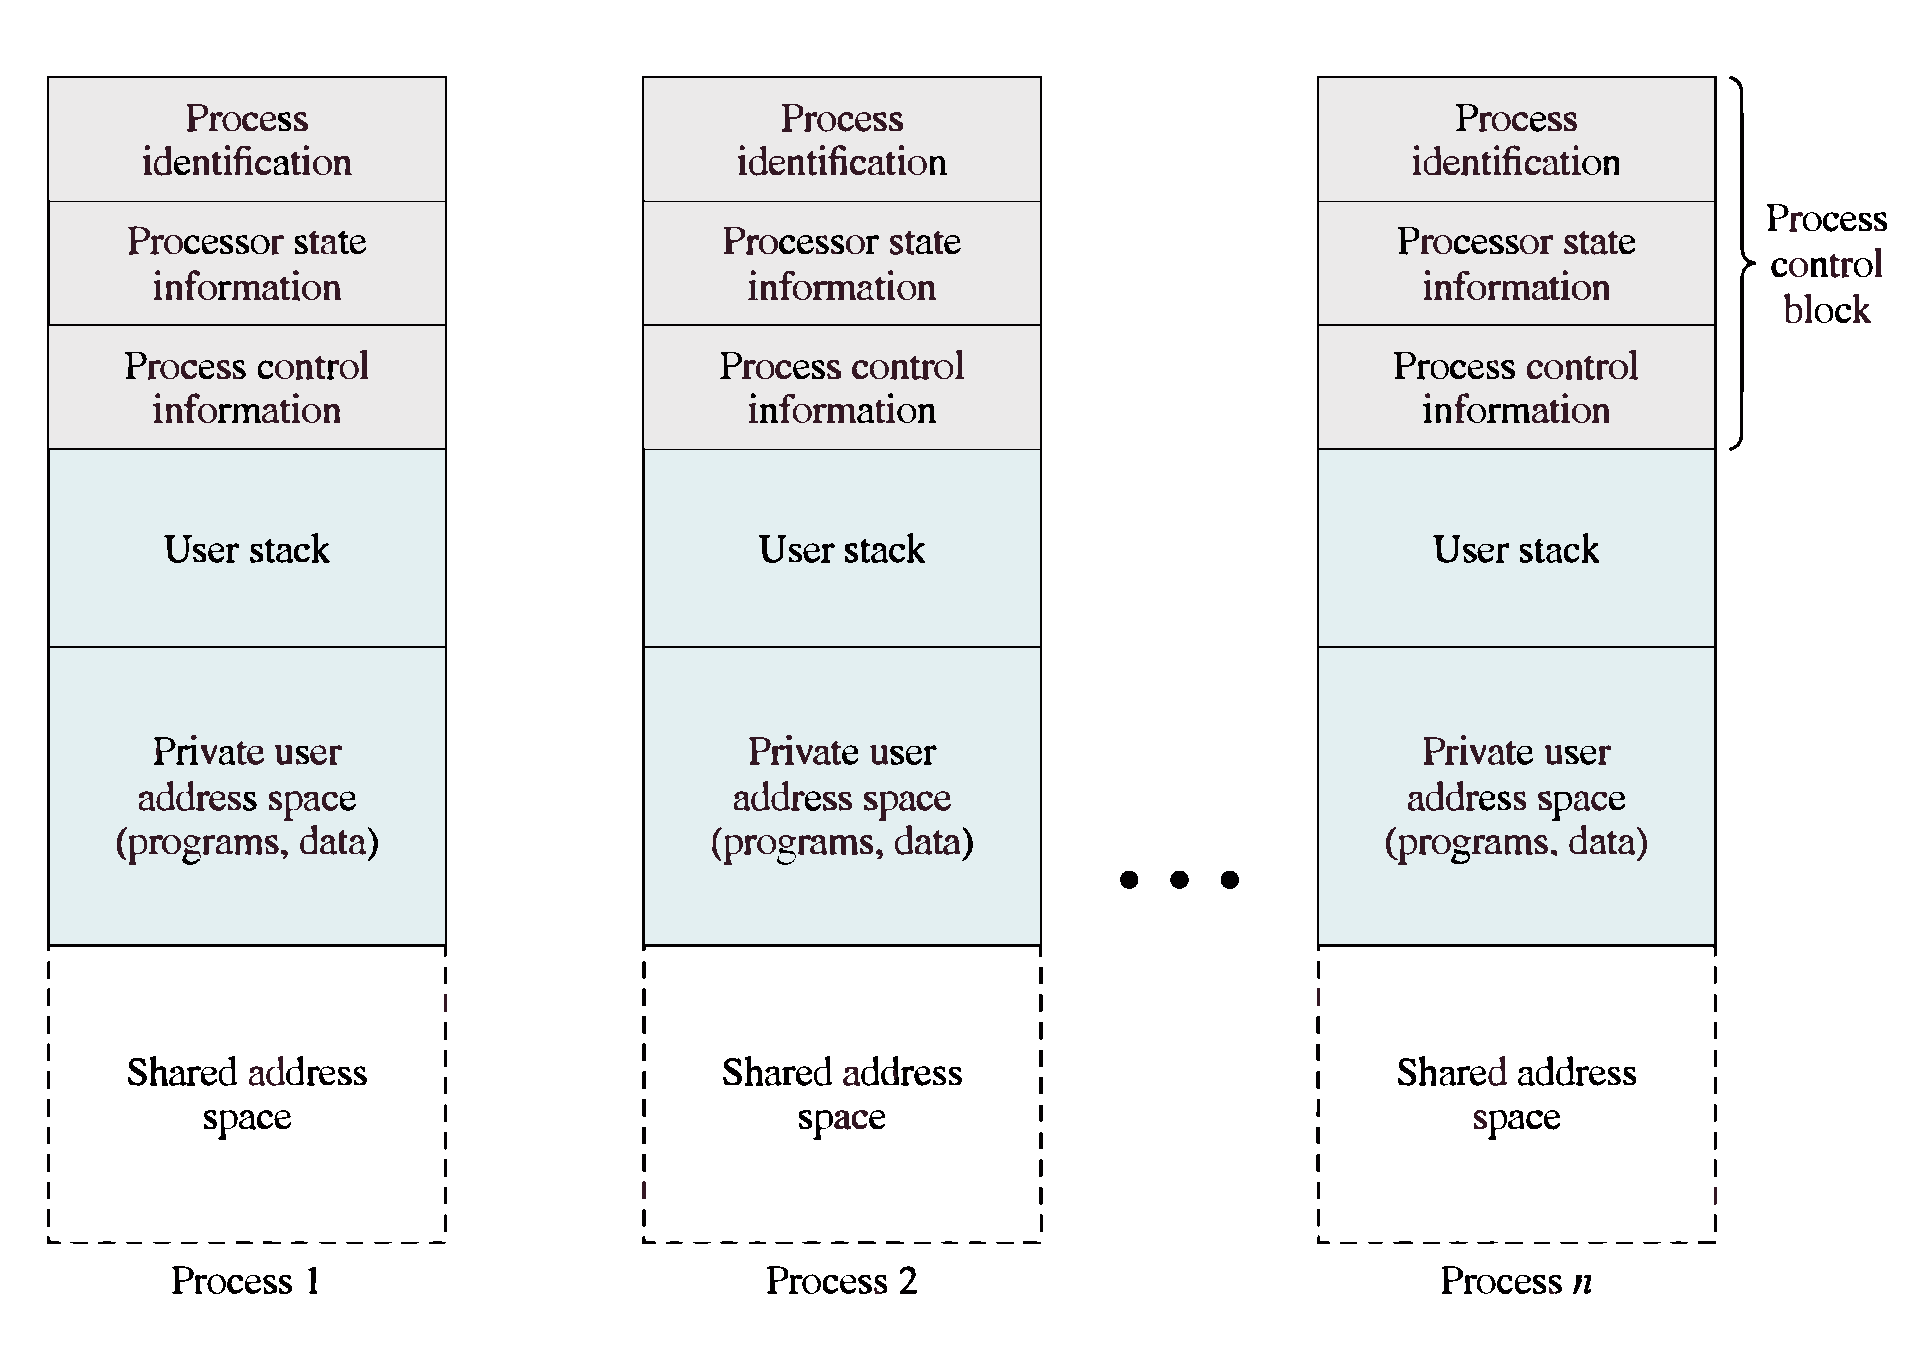
\includegraphics[width=0.90\textwidth]{assets/Proceso.eps}
    \end{center}
    \caption{Procesos en Memoria Virtual}\label{fig:1}
\end{figure}
\pagebreak

\subsection{Contexto de un proceso}
\begin{itemize}
    \item Inclute toda la informacion que el So necesita para administrar el proceso, y la CPu para ejecutarlo correctamente.
    \item Son parte del contexto, los registros de cpu, inclusive cl contador del programa, prioridad, etc.
\end{itemize}
\subsubsection{Context Switch}
\begin{itemize}
    \item Se produce cuando la cpu cambia de un proceso a otro.
    \item Se debe resguardar el contexto del proceso saliente, que pasa a espera y retornara despues a la CPU.
    \item Se debe cargar el contexto del nuevo proceso y comenzar desde la instruccion siguiente a la ultima ejecutada en dicho contexto.
    \item Es tiempo no productivo de la CPU.
    \item El tiempo que consume depende del soporte de HW.
\end{itemize}
\begin{figure}[ht]
    \begin{center}
        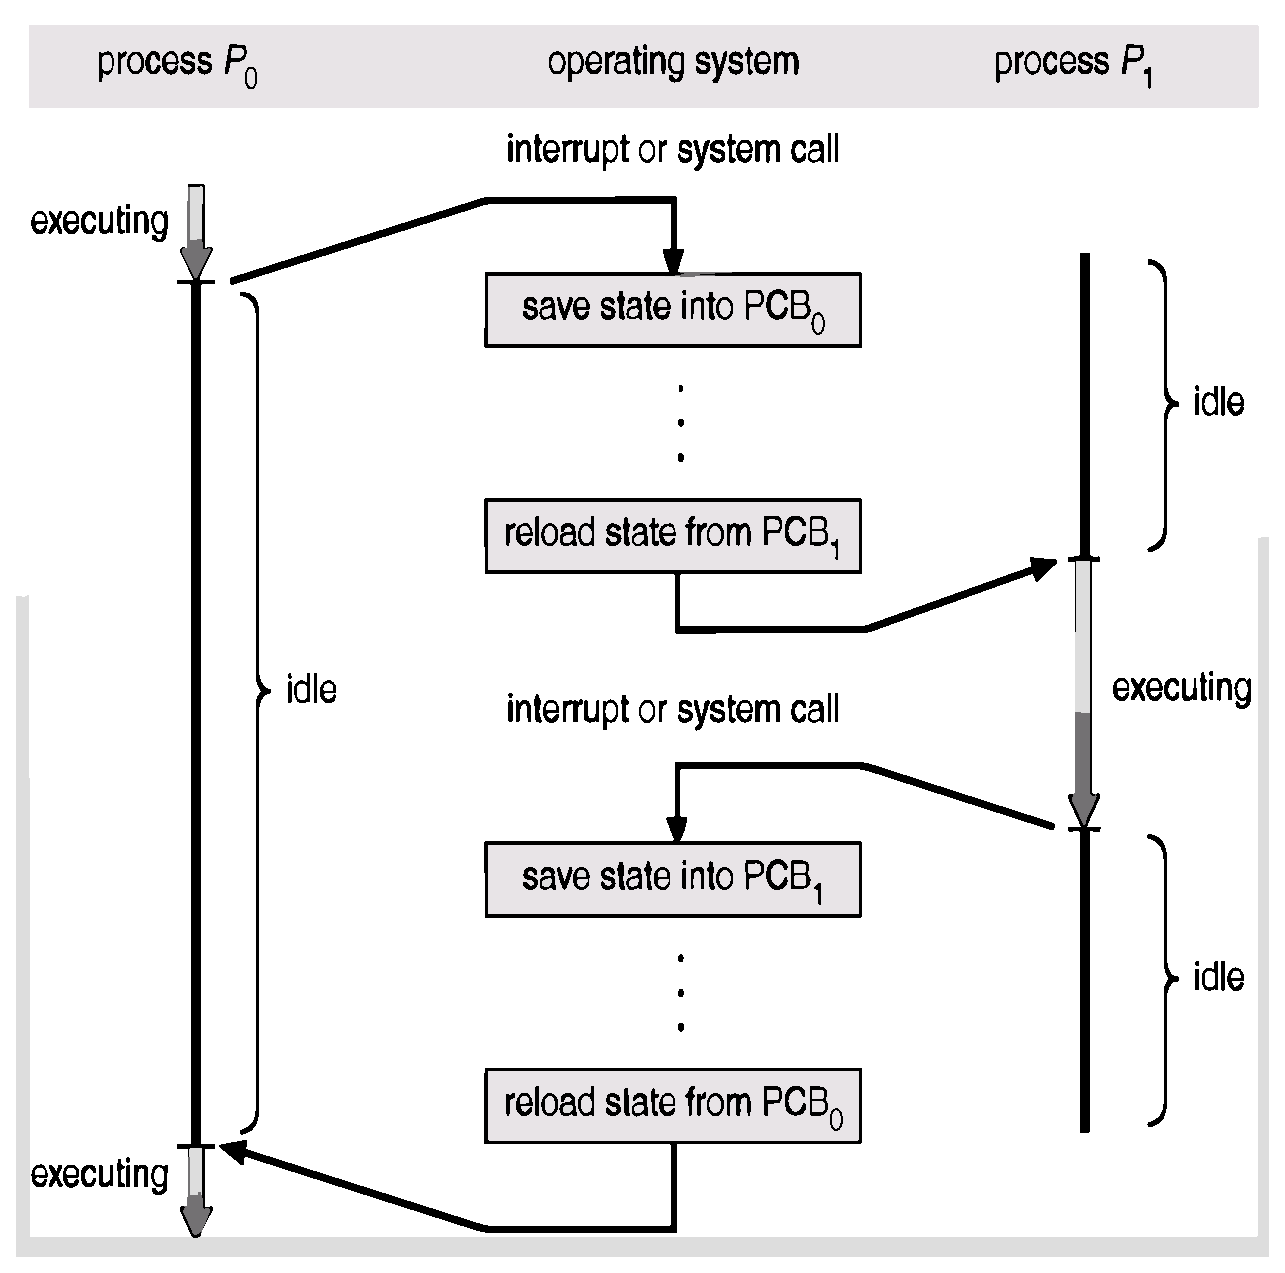
\includegraphics[width=0.65\textwidth]{assets/ContextSwitch.eps}
    \end{center}
    \caption{Context Switch}\label{fig:}
\end{figure}

\subsection{Ejecucion del Kernel}
\begin{itemize}
    \item El kernel es un conjunto de modulos de software.
    \item Se ejecuta en el procesdor como cualquier otro proceso.
    \item Existen diferentes enfoques de diseño:
\end{itemize}
\subsubsection{El kernel como entidad independiente}
\begin{itemize}
    \item El kernel se ejecuta fuera de todo proceso.
    \item El kernel se ejecuta fuera de todo proceso.
    \item Cuando un proceso es interrumpido o realiza una System Call, el contexto del proceso se salva y el control se pasa al Kernel del SO.
    \item el Kernel posee su propia region de memoria y su propio Stack.
    \item Finalizada su actividad, le devuelve el control al proceso.
    \item El kernel NO es un proceso.
    \item Se ejecuta como una entidad independiente en modo privilegiado.
\end{itemize}
\begin{figure}[h]
    \begin{center}
        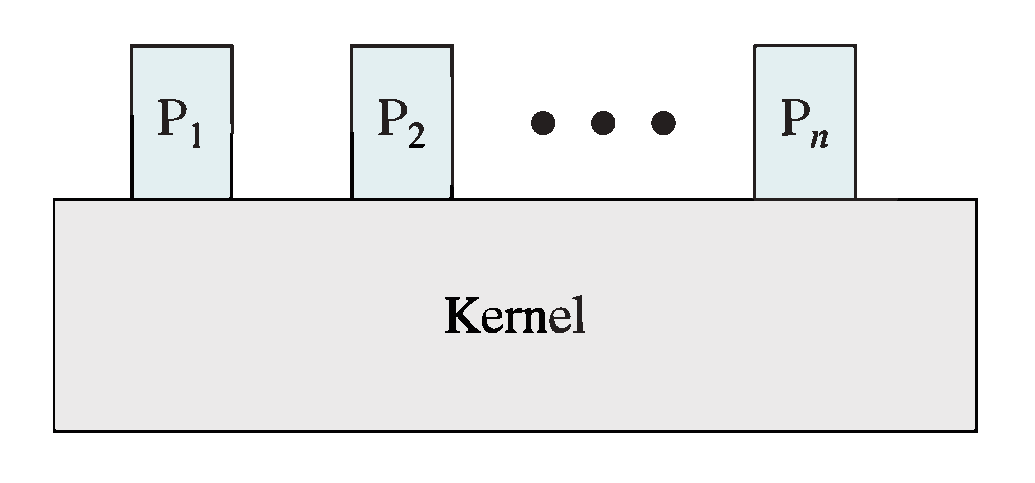
\includegraphics[width=0.45\textwidth]{assets/Kernel1.eps}
    \end{center}
    \caption{Kernel como identidad independiente}\label{fig:}
\end{figure}

\vspace{2cm}

\subsubsection{El kernel "dentro" del proceso}
\begin{itemize}
    \item El codigo del Kernel se encuentra dentro del espacio de direcciones de cada proceso.
    \item El Kernel se ejecuta en el mismo contexto que algun proceso de usuario.
    \item El Kernel se puede ver como una coleccion de rutinas que el proceso utiliza.
    \item Dentro de un proceso se encuentra el codigo del programa y el codigo de los modulos SW del SO (kernel).
    \item Cada proceso tiene un stack en modo usuario y otro en modo Kernel. 
    \item Cada interrupcion es atendida en el contexto del proceso que se encontraba en ejecucion(en modo kernel).
    \item Si el SO determina que el proceso debe seguir ejecutandose luego de atender la interrupcion, cambia a modo usuario y devuelve el control.
\end{itemize}
\vspace{2cm}
\begin{figure}[ht]
    \begin{center}
        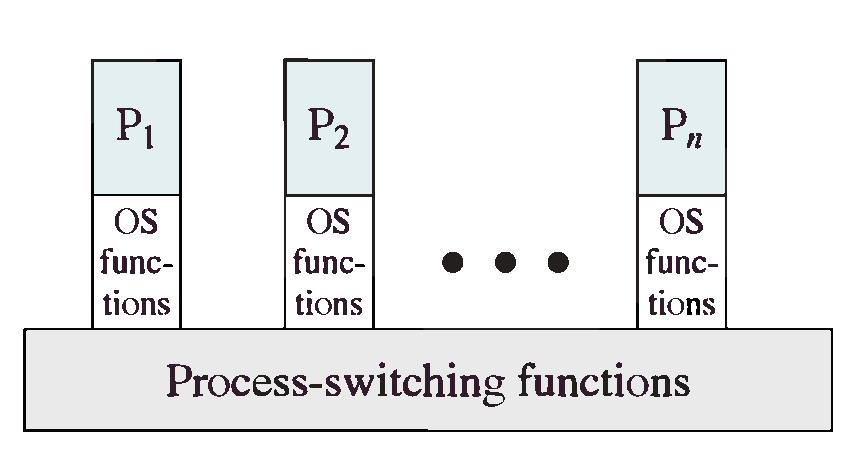
\includegraphics[width=0.50\textwidth]{assets/Kernel2.eps}
    \end{center}
    \caption{Kernel dentro del proceso}\label{fig:}
\end{figure}

\subsection{Estados de un Proceso}
En su estado de vida, un proceso pasa por diferentes estados:
\begin{itemize}
    \item \textbf{Nuevo (new)}.
    \item \textbf{Listo (ready)}.
    \item \textbf{Ejecucion (running)}.
    \item \textbf{En espera/bloqueado (waiting/blocked)}.
    \item \textbf{Terminado (terminated)}.
\end{itemize}

\begin{figure}[h]
    \begin{center}
        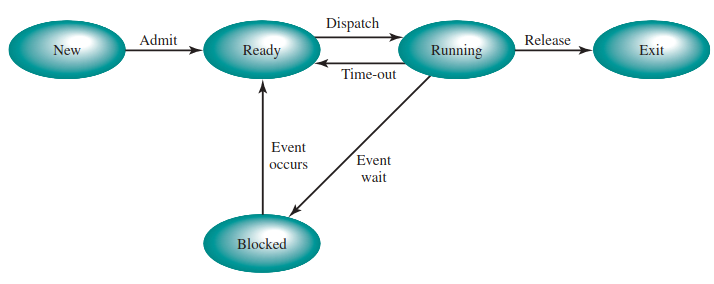
\includegraphics[width=0.90\textwidth]{assets/estados.png}
    \end{center}
    \caption{Estados de un proceso}\label{fig:}
\end{figure}

\pagebreak
\subsection{Colas en la planificacion de procesos}
\begin{itemize}
    \item Para realizar al planificacion, el SO utiliza la PCB de cada proceso como una abstraccion del mismo.
    \item Las PCB se enlazan en colas siguiendo un orden determinado.
\end{itemize}
\begin{figure}[h]
    \begin{center}
        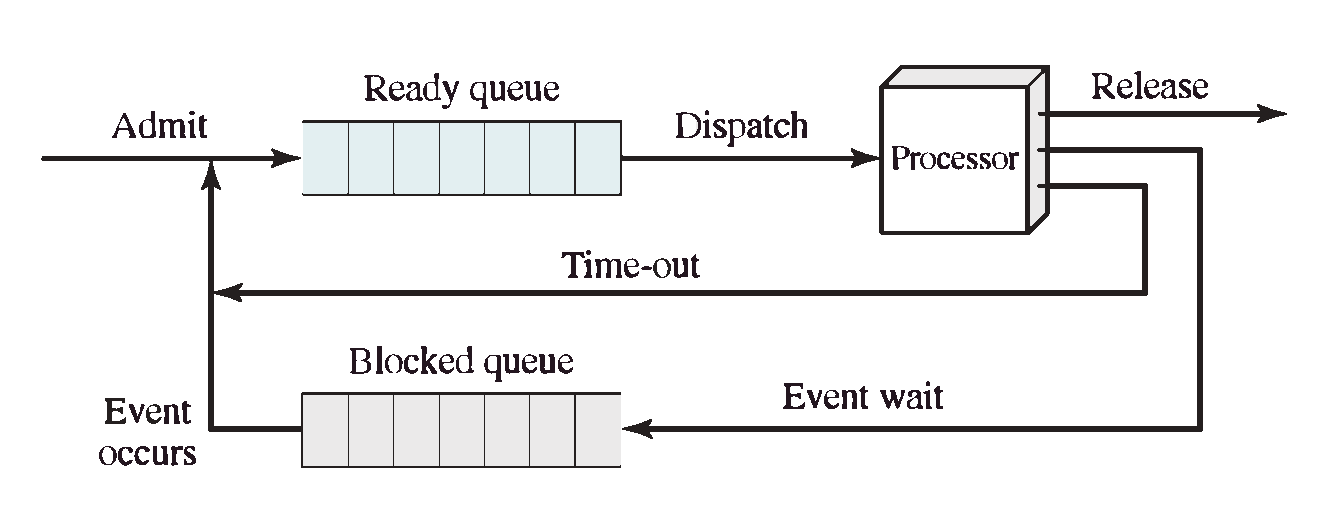
\includegraphics[width=0.75\textwidth]{assets/ProcessQueue.eps}
    \end{center}
    \caption{Colas de Planificacion}\label{fig:}
\end{figure}

\subsubsection{Modulos de la planificacion}
\begin{itemize}
    \item Son modulos de SW del Kernel que realizan distiintas tareas asociadas a la planificacion.
    \item Se ejecutan ante determinados eventos:
    \begin{itemize}
        \item Creacion/Terminacion de procesos.
        \item Eventos de sincronizacion.
        \item Finalizacion de lapso de tiempo.
        \item Etc.
    \end{itemize}
    \item Existen 3 schedulers:
        \begin{itemize}
            \item \textbf{Long Term Scheduler} 
            \item \textbf{Short Term Scheduler} 
            \item \textbf{Medium Term Scheduler} 
        \end{itemize}
    \item \textbf{Dispatcher:} realiza el cambio de contexto, cambio de modo ejecucion y despacha el proceso elegido por el Short Term.
    \item \textbf{Loader} carga en memoria el proceso elegido por el long term.
\end{itemize}
\begin{figure}[h]
    \begin{center}
        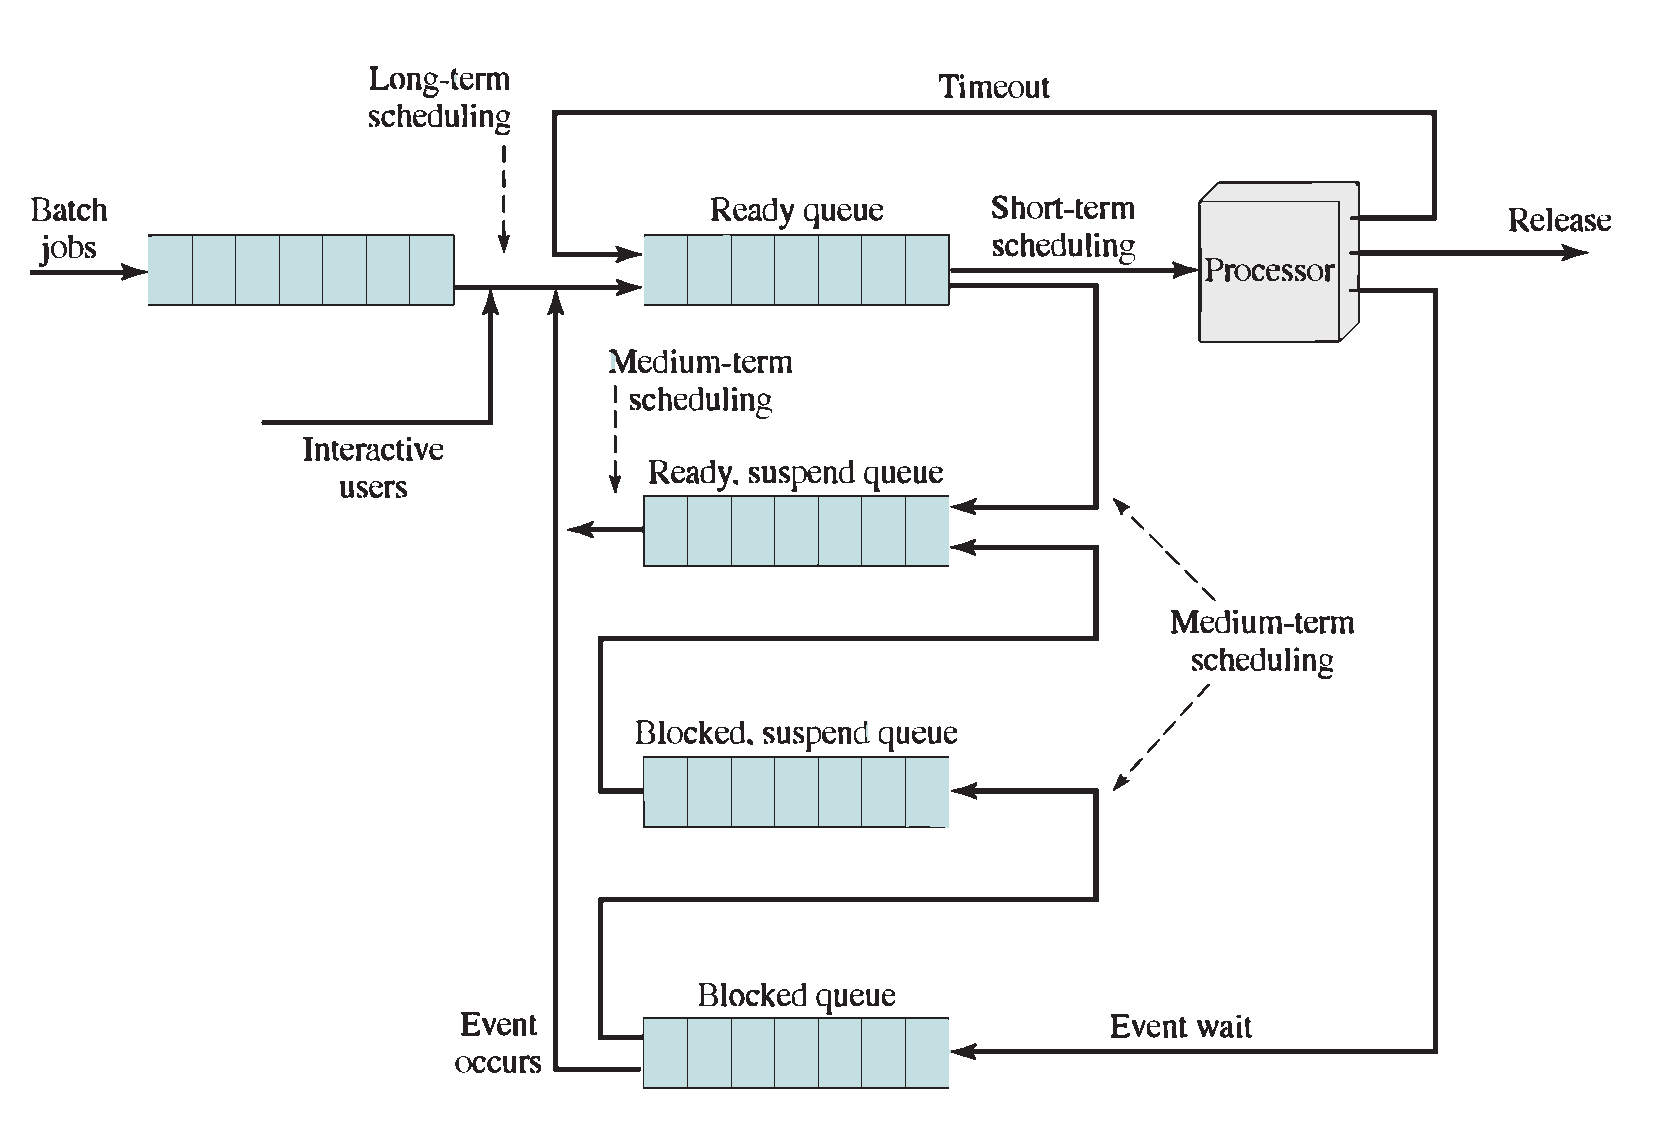
\includegraphics[width=0.90\textwidth]{assets/Schedulers.eps}
    \end{center}
    \caption{Schedulers}\label{fig:}
\end{figure}


\subsubsection{Schedulers}
\begin{itemize}
    \item \textbf{Long Term Scheduler}
        \begin{itemize}
            \item Controla el grado de multiprogramacion.
            \item Puede no existir este scheduler y absorber esta tarea el de short term.
        \end{itemize}
    \item \textbf{Medium Term Scheduler}
        \begin{itemize}
    \item Si es necesario, reduce el grado de multiprogramacion.
    \item Saca temporalmente de memoria los procesos que sea necesario para mantener el equilibrio del sistema.
\end{itemize}
\item \textbf{Short Term Scheduler}
\begin{itemize}
    \item Decide a cual de los procesos en la cola de listos se elige para que use la CPU.
    \item Terminos asociados: apropiativo, no apropiativo, algoritmo de scheduling.
\end{itemize}
\end{itemize}

\begin{figure}[ht]
    \begin{center}
        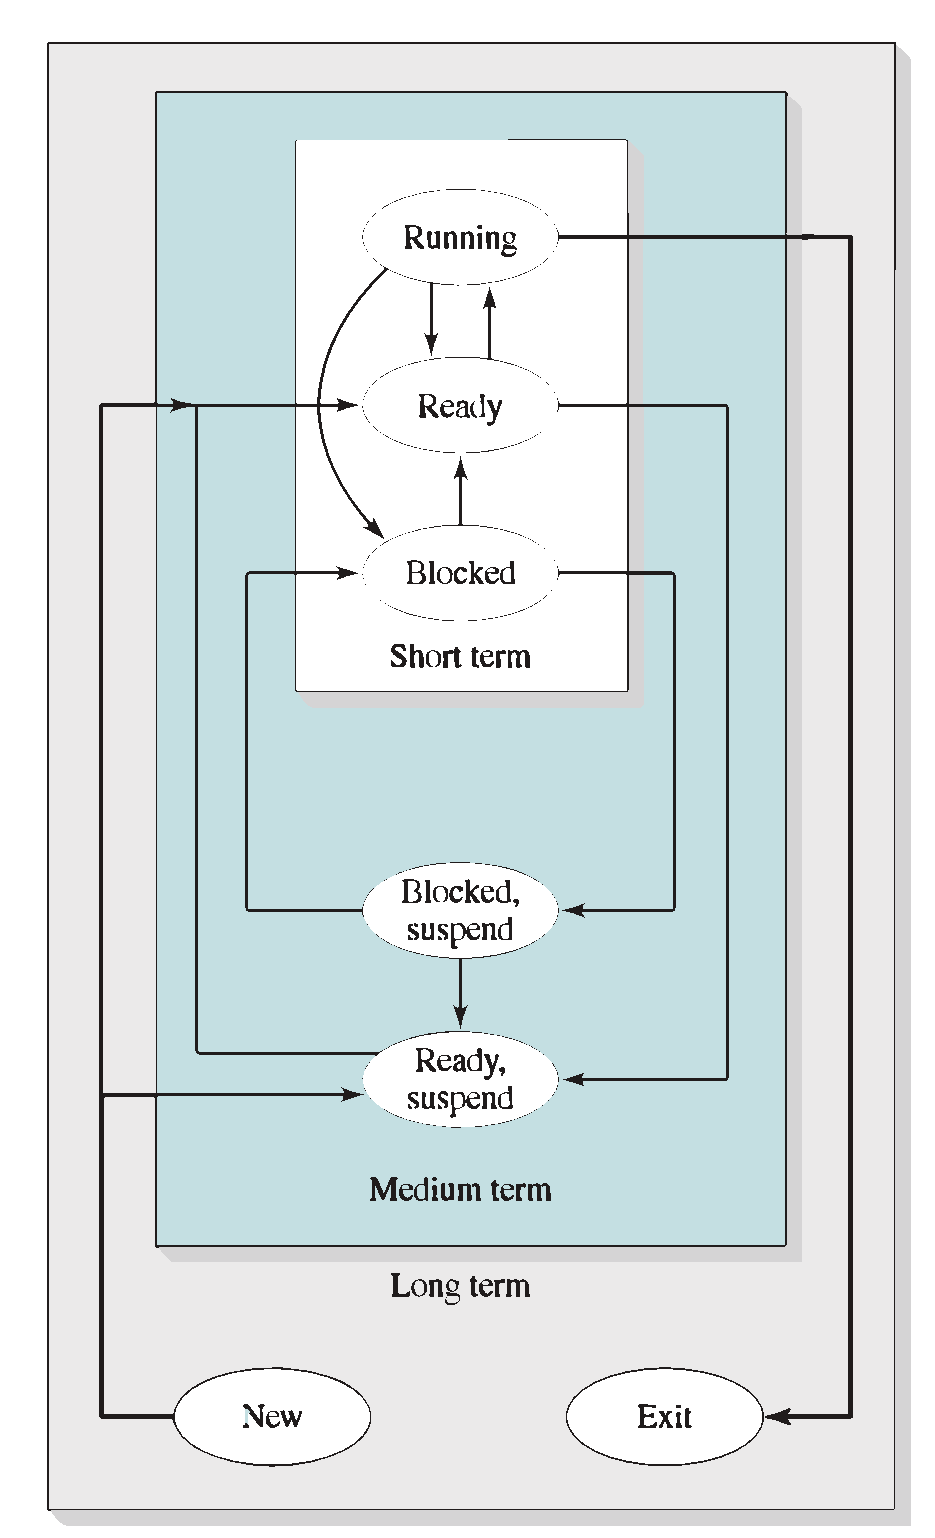
\includegraphics[width=0.50\textwidth]{assets/Schedulers2.pdf}
    \end{center}
    \caption{Schedulers}\label{fig:5}
\end{figure}

\subsection{Estados de los procesos}
\begin{itemize}
    \item \textbf{Nuevo (new):}
        \begin{itemize}
            \item Un usuario "dispara" el proceso. Un proceso es creado por otro proceso: su proceso padre.
            \item En este estado, se crean las estructuras asociadas, y el proceso queda en la cola de procesos, normalmente en espera de ser cargado en memoria.
        \end{itemize}
    \item \textbf{Listo (ready):}
        \begin{itemize}
            \item Luego que el Long Term Scheduler elige al proceo para cargarlo en memoria, el proceso queda en estado listo.
            \item El proceso solo necesita que se le asigne CPU.
            \item Esta en la cola de procesos listos (ready queue).
        \end{itemize}
    \item \textbf{Ejecucion (running):}
        \begin{itemize}
            \item El Long Term Scheduler lo eligio para asignarle CPU.
            \item Tendra la CPU hasta que se termine el periodo de tiempo asignado, termine o hasta que necesite realizar alguna operacion de E/S.
        \end{itemize}
    \item \textbf{En espera/bloqueado (waiting/blocked):}
    \begin{itemize}
        \item El proceso necesita que se cumpla el evento esperado para continuar.
        \item El evento puede ser la terminacion de una E/S solicitada, o la llegada de una senal por parte de otro proceso.
        \item Sigue en memoria, pero no tiene la CPU.
        \item Sigue en memoria, pero no tiene la CPU.
    \end{itemize}
\end{itemize}

\subsection{Comportamiento de los procesos}
\begin{itemize}
    \item \textbf{CPU-bound:} mayor parte del tiempo utilizando la CPU.
    \item \textbf{I/O bound:} mayor parte del tiempo eeperando por I/O.
\end{itemize}

\subsection{Algoritmos de Planificacion}
\begin{itemize}
    \item \textbf{Planificacion:} necesidad de determinar cual de todos los procesos que estan listos para ejecutarse, sera el proximo en ejecutarse.
    \item \textbf{Algoritmos Preemmtive:} existen situaciones que hacen que el proceso en ejecucion sea expulsado de la CPU.
    \item \textbf{Algoritmos No Preemmtive:} los procesos se ejecutan hasta que el mismo (por su propia cuenta) abandone la CPU.
\end{itemize}

\subsection{Algoritmos segun el tipo de proceso}
\subsubsection{Procesos Batch}
\begin{itemize}
    \item No existen usuarios que esperen una respuesta en la termina.
    \item Se pueden utilizar algoritmos no apropiativos.
    \item Metas propias de este tipo de algoritmos:
        \begin{itemize}
            \item Rendimiento: Maximizar  numero de trabajos por hora.
            \item Tiempo de Retorno: Minimizar los tiempos entre el comienzo y la finalizacion.
            \item El tiempo de espera se puede ver afectado.
            \item Uso de la CPU: Mantener la CPU ocupada la mayor cantidad de tiempo posible.
        \end{itemize}
\end{itemize}

\subsubsection{Procesos Interactivos}
\begin{itemize}
    \item No solo interaccion con los usuarios.
    \item Son necesarios algoritmos apropiativos para evitar que un proceso acapare la CPU.
    \item Metas propias de este tipo de algoritmos:
    \begin{itemize}
        \item Tempo de respuesta: Responder a peticiones con rapidez.
        \item Proporcionalidad: Cumplir con expectativas de los usuarios. Por ej: al poner STOP al reproductor de musica, debe dejar de ser reproducida en un tiempo corto.
    \end{itemize}
\end{itemize}

\subsection{Creacion de procesos}
\begin{itemize}
    \item Un proceso es creaado por otro proceso.
    \item Un proceso padre tiene uno o mas procesos hijos.
    \item Se forma un arbol de procesos.
    \item Actividades en la creacion:
    \begin{itemize}
        \item Crear la PCB.
        \item Asignar PID unico.
        \item Asignarle memoria para regiones.
        \item Crear estructuras de datos asociadas.
    \end{itemize}
\end{itemize}

\subsubsection{Relacion entre procesos padre e hijo}
\begin{itemize}
    \item El padre puede continuar ejcutandose concurrentemente con su hijo.
    \item El padre puede esperar a que el/los procesos hijos terminen para continuar la ejecucion.
\end{itemize}

\section{Memoria}

\subsection{Rol del Sistema Operativo}
El SO debe:
\begin{itemize}
    \item Llevar un registro de las partes de memoria que se están utilizando y de aquellas que no.
    \item Asignar espacio en memoria principal a los procesos cuando estos lo necesitan.
    \item Liberar espacio de memoria asignada a procesos que han terminado.
    \item Lograr que el programador se abstraiga de la asignación de los programas.
    \item Brindar seguridad entre los procesos para que unos no accedan a secciones privadas de otros.
    \item Brindar la posibilidad de acceso compartido a determinadas secciones de la memoria.
    \item Garantizar el rendimiento.
\end{itemize}

\subsection{Requisitos}
\begin{itemize}
    \item \textbf{Reubicación}
    \begin{itemize}
        \item El programador no debe ocuparse de conocer dónde será colocado en la memoria RAM.
        \item Mientras un proceso se ejecuta, puede ser sacado y traído a la memoria (swap) y, posiblemente, colocarse en diferentes direcciones.
        \item Las referencias a la memoria se deben "traducir" según la ubicación actual del proceso.
    \end{itemize}
    \item \textbf{Protección}
    \begin{itemize}
        \item Los procesos NO deben referenciar/acceder a direcciones de memoria de otros procesos (salvo que tengan permiso).
        \item El chequeo se debe realizar durante la ejecución.
    \end{itemize}
\item \textbf{Compartición}
    \begin{itemize}
        \item Permitir que varios procesos accedan a la misma porción de memoria.
        \item Permitir un mejor uso de la memoria principal, evitando copias innecesarias (repetidas) de instrucciones.
    \end{itemize}
\end{itemize}

\subsection{Direcciones}
\subsubsection{Espacio de direcciones}
\begin{itemize}
    \item Rango de direcciones (a memoria) posibles que un proceso puede utilizar para direccionar sus instrucciones y datos.
    \item Es independiente de la ubicación "real" del proceso en la memoria RAM.
\end{itemize}

\subsection{Tipos de direcciones}
\begin{itemize}
    \item \textbf{Lógicas/Virtuales}
    \begin{itemize}
        \item Referencia a una localidad de memoria.
        \item Representa una dirección en el "Espacio de Direcciones del Proceso".
    \end{itemize}
    \textbf{Físicas}
    \begin{itemize}
        \item Referencia una localidad en la memoria principal.
    \end{itemize}
\end{itemize}
Es necesario algún tipo de conversión de direcciones lógicas a físicas y viceversa.
\subsubsection{Conversión de Direcciones}
Una forma simple de realizar la conversión es utilizando registros auxiliares.
\begin{itemize}
    \item \textbf{Registro Base:} dirección de comienzo del Espacio de Direcciones del proceso en la memoria principal.
    \item \textbf{Registro Límite} dirección final del proceso o medida del proceso.
    \item Ambos valores se fijan cuando el espacio de direcciones del proceso es cargado a memoria.
    \item Varían entre procesos.
\end{itemize}
    Si la conversión se realiza en tiempo de ejecución, las direcciones lógicas se denominan \textbf{direcciones virtuales}, y son diferentes a las físicas.
En este caso, el mapeo entre ambos tipos de direcciones se realiza por hardware, mediante la \textbf{Memory Management Unit (MMU)}.
\begin{figure}
    \begin{center}
        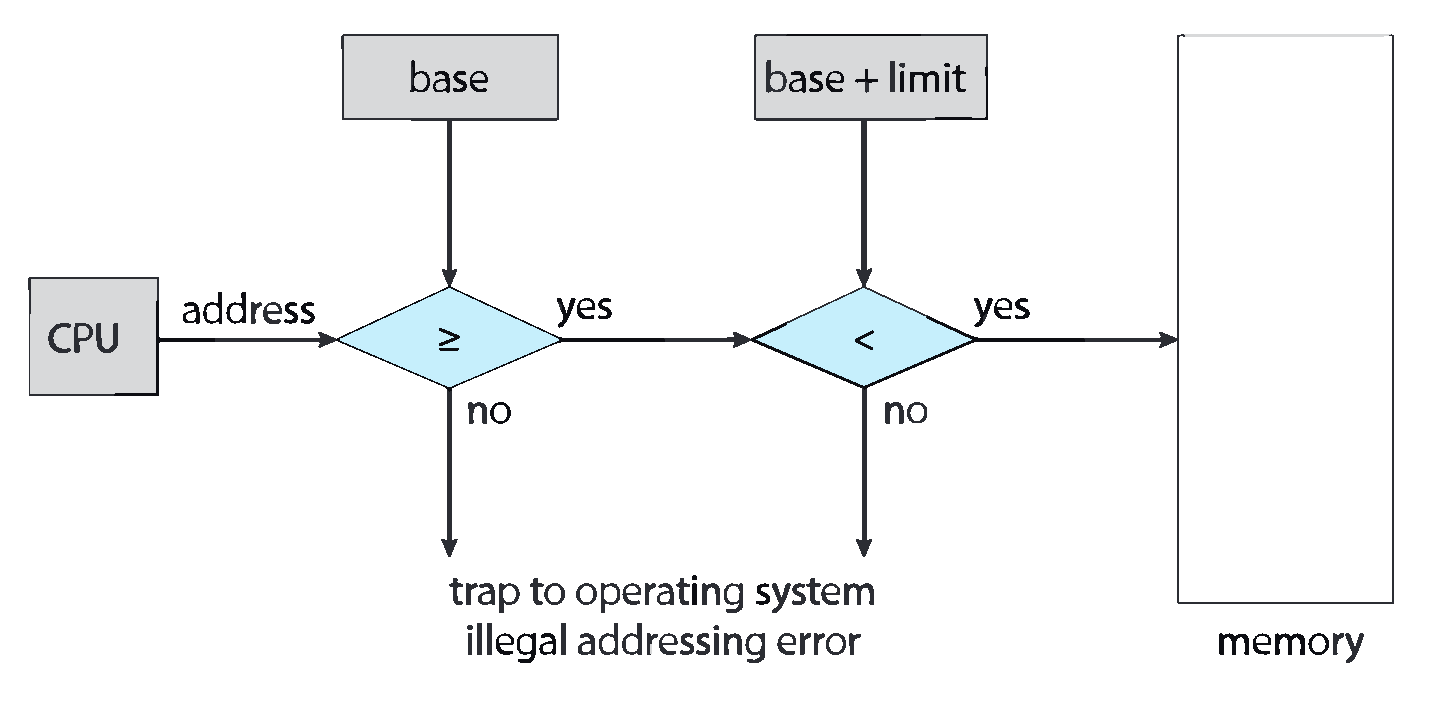
\includegraphics[width=0.75\textwidth]{assets/ConversionDirecciones.pdf}
    \end{center}
    \caption{Protección de direcciones mediante registros base y límite.}\label{fig:69}
\end{figure}
\subsection{Memory Management Unit (MMU)}
\begin{itemize}
    \item Es un dispositivo de hardware que mapea direcciones virtuales a físicas.
    \item Es parte de la CPU.
    \item Reprogramarla es una operación privilegiada.
    \item El valor en el "registro de realocación" es sumado a cada dirección generada por el proceso de usuario al momento de acceder a la memoria.
    \item Los procesos solo utilizan direcciones virtuales.
\end{itemize}
\begin{figure}[h]
    \begin{center}
        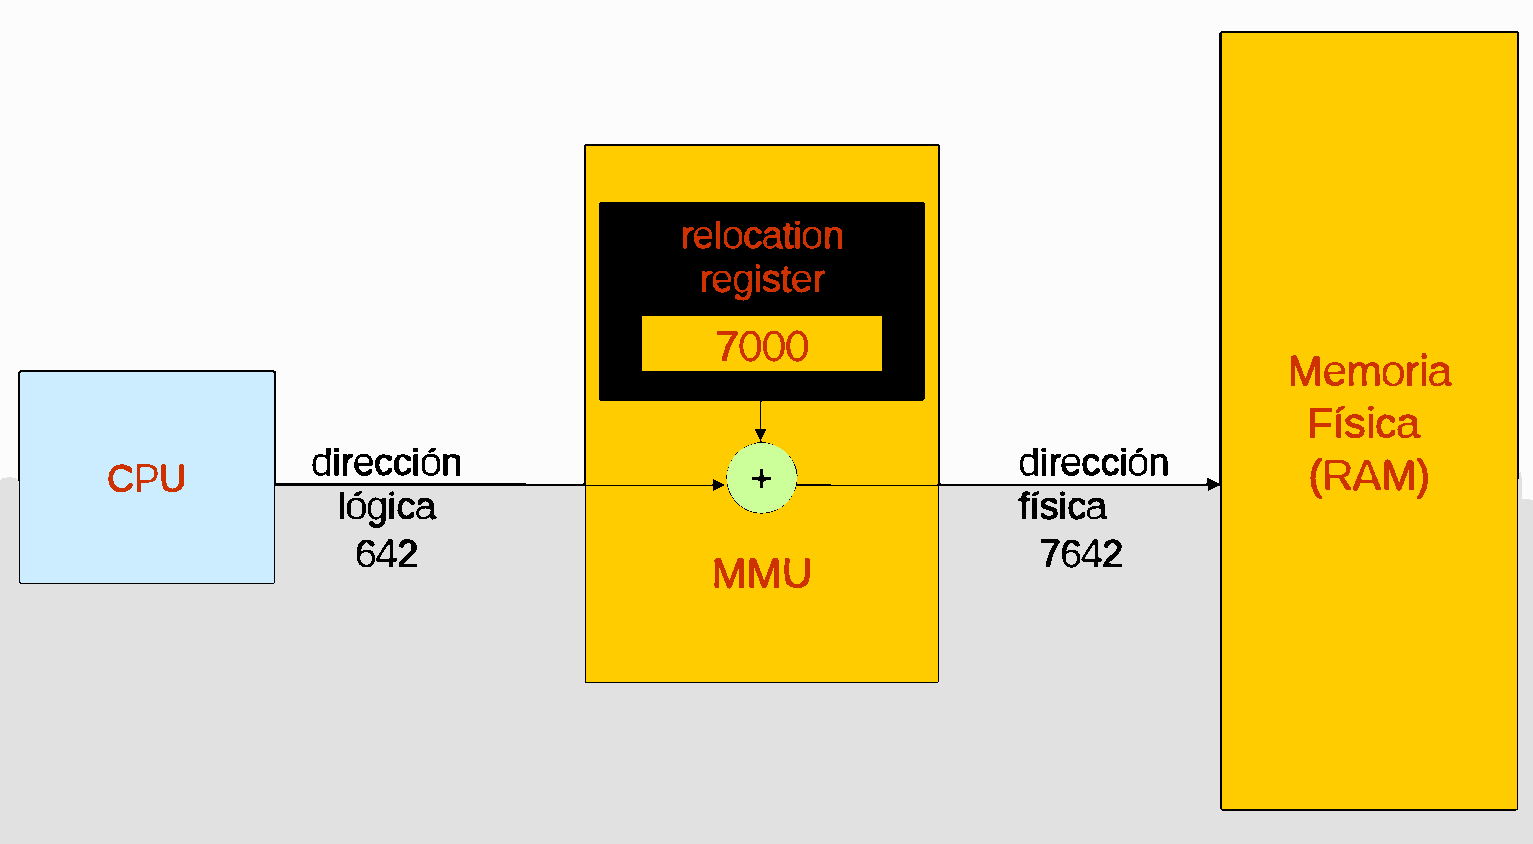
\includegraphics[width=0.70\textwidth]{assets/MMU.pdf}
    \end{center}
    \caption{Funcionamiento de la MMU}\label{fig:}
\end{figure}

\subsection{Mecanismos de asignación de memoria}
\begin{itemize}
    \item \textbf{Particiones Fijas}
    \begin{itemize}
        \item La memoria se divide en particiones o regiones de tamaño fijo (del mismo tamaño o no).
        \item Alojan un proceso cada una.
        \item Cada proceso se coloca de acuerdo a algún criterio (worst-fit, best-fit, etc).
    \end{itemize}
    \item \textbf{Particiones Dinámicas}
    \begin{itemize}
        \item Las particiones varían en tamaño y número.
        \item Alojan un proceso cada una.
        \item Cada partición se genera en forma dinámica, del tamaño exacto que necesita el proceso.
    \end{itemize}
\end{itemize}

\subsection{Fragmentación}
La \textbf{fragmentación} se produce cuando una alocalidad de memoria no puede ser utilizada por no encontrarse en forma continua.
Existen dos tipos:
\begin{itemize}
    \item \textbf{Fragmentación Interna}
    \begin{itemize}
        \item Se produce en el esquema de particiones fijas.
        \item Es la porción de la partición que queda sin utilizar.
    \end{itemize}
    \item \textbf{Fragmentación Externa}
    \begin{itemize}
        \item Se produce en el esquema de particiones dinámicas.
        \item Son huecos que van quedando en la memoria a medida que los procesos finalizan.
        \item Al no encontrarse en forma contigua, puede darse el caso de que tengamos memoria libre para alojar un proceso, pero que no la podamos utilizar.
        \item Puede solucionarse utilizando la \textbf{compactación}.
    \end{itemize}
\end{itemize}

\subsection{Paginación}
\begin{itemize}
    \item La memoria física es dividida lógicamente en pequeños trozos de igual tamaño llamados \textbf{Marcos}.
    \item La memoria lógica (espacio de direcciones) es dividida en trozos de igual tamaño que los marcos, llamados \textbf{Páginas}.
    \item El SO debe mantener una tabla de páginas por cada proceso, donde cada entrada contiene (entre otras), el Marco en el que se coloca cada página.
    \item La dirección lógica se interpreta como un número de página y un desplazamiento dentro de la misma.
\end{itemize}
\begin{figure}[h]
    \begin{center}
        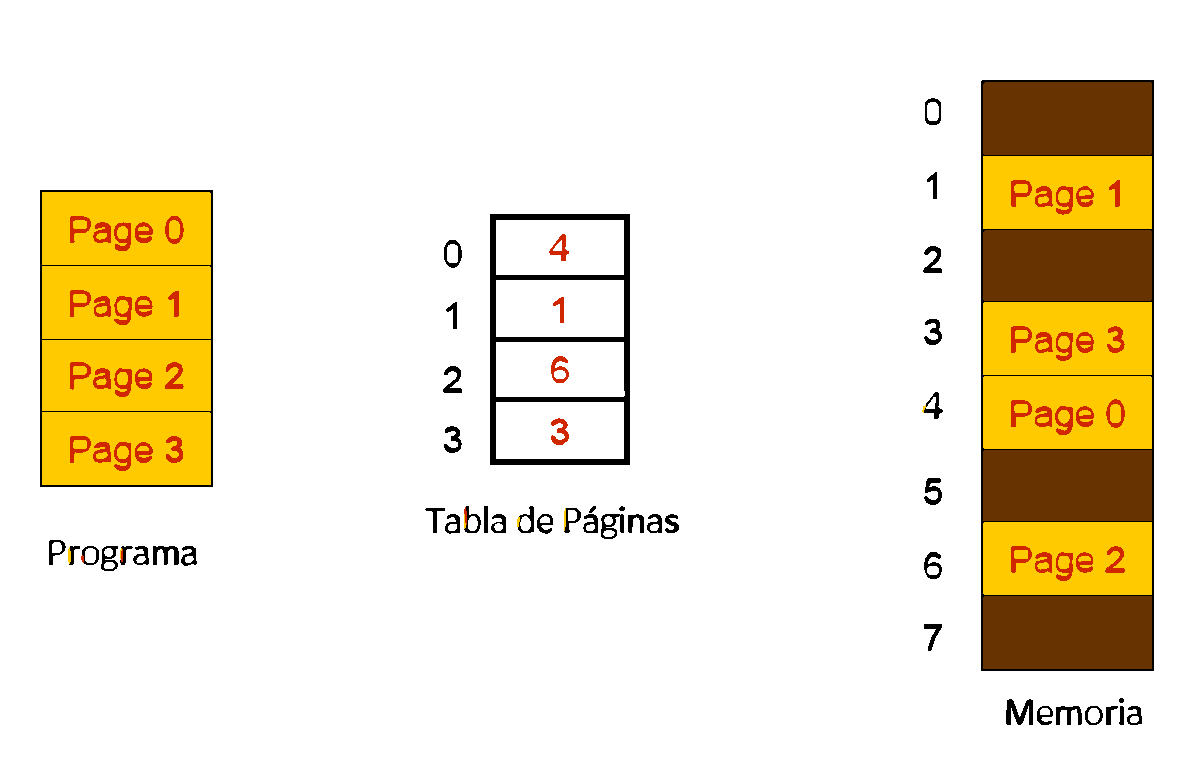
\includegraphics[width=0.70\textwidth]{assets/Paging.pdf}
        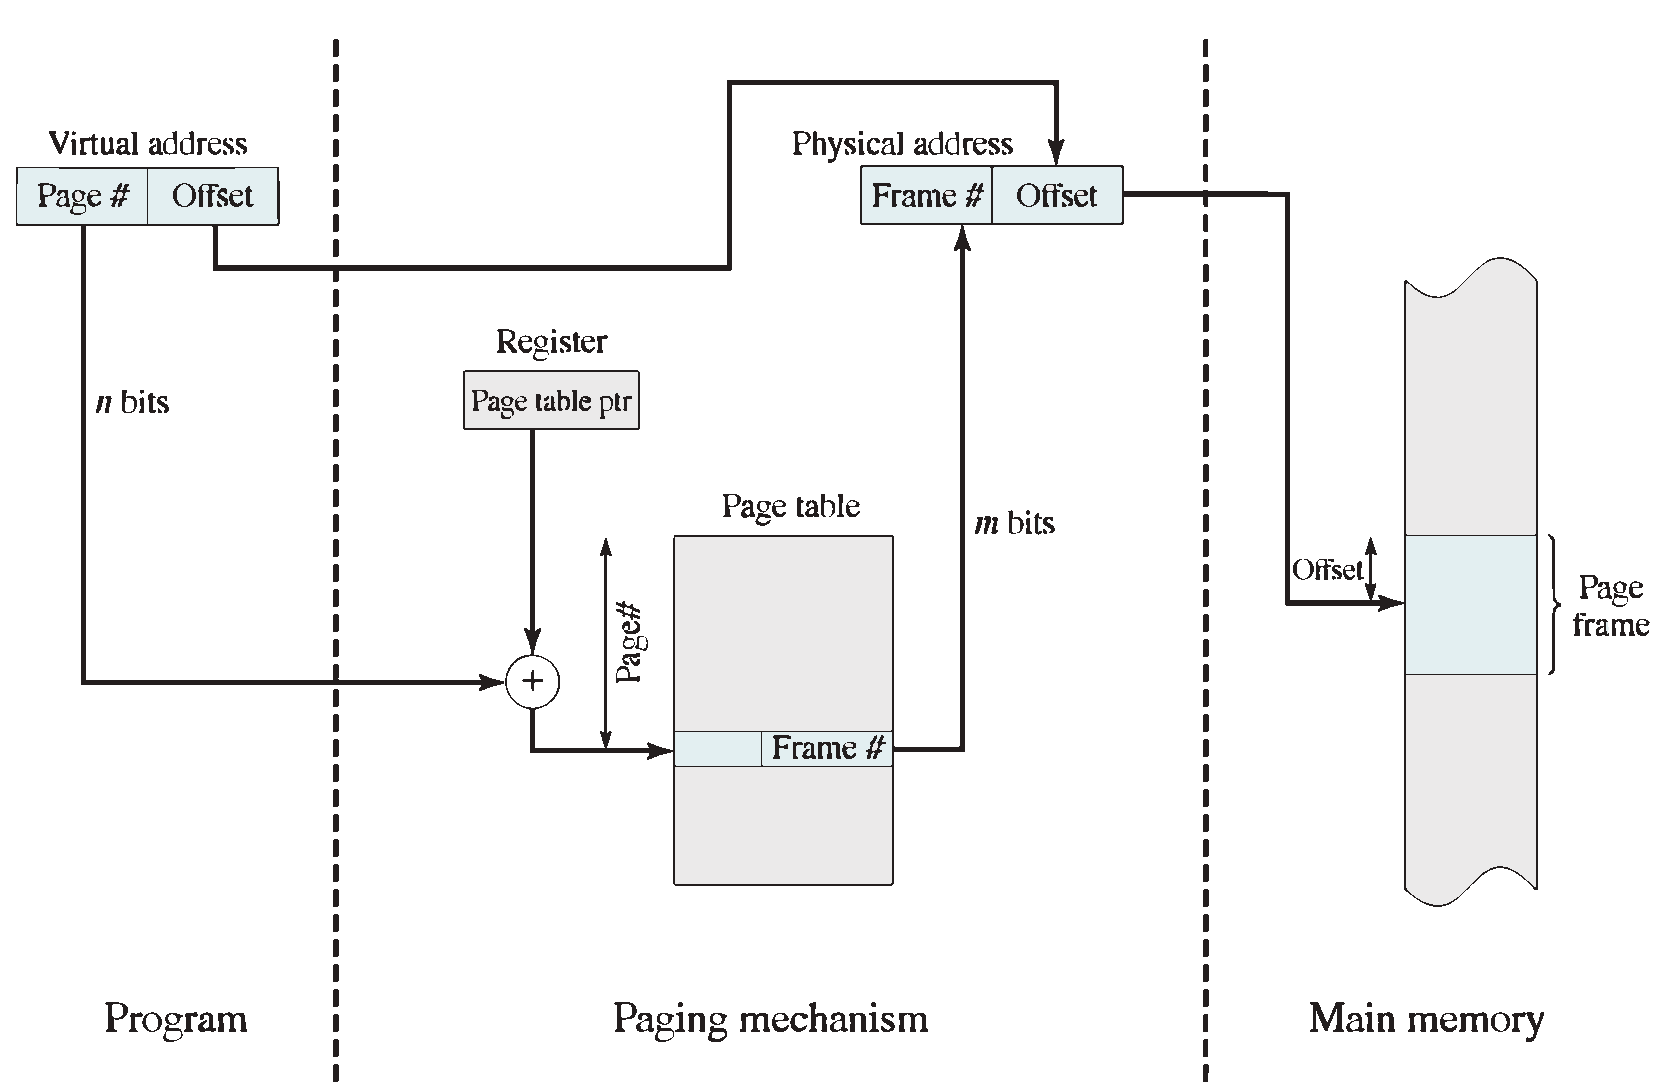
\includegraphics[width=0.80\textwidth]{assets/PagingTraslation.pdf}
    \end{center}
    \caption{Ejemplo de Paginación}\label{fig:}
\end{figure}
\pagebreak

\subsection{Segmentación}
\begin{itemize}
    \item Esquema que se asemeja a la "visión del usuario". El programa se divide en partes/secciones.
    \item Un programa es una colección de segmentos. Un segmento es una unidad lógica, como Programa Principal, Procedimientos y Funciones, variables locales/globales, etc.
    \item Puede causar fragmentación.
    \item Todos los segmentos de un programa pueden no tener el mismo tamaño.
    \item Las direcciones lógicas consisten en 2 partes:
    \begin{itemize}
        \item Selector de Segmento.
        \item Desplazamiento dentro del segmento. 
    \end{itemize}
    \item \textbf{Tabla de Segmentos:} permite mapear la dirección lógica a física. Cada entrada contiene:
    \begin{itemize}
        \item Base: Dirección física del comienzo del segmento.
        \item Límite: Tamaño del segmento.
    \end{itemize}
    \item Segment-Table base register (STBR): contiene la dirección de la tabla de segmentos.
    \item Segment-Table length register (STLR): contiene la cantidad de segmentos de un programa.
\end{itemize}
%it just works
\vspace{-0.5cm}
\begin{figure}[h]
    \begin{center}
        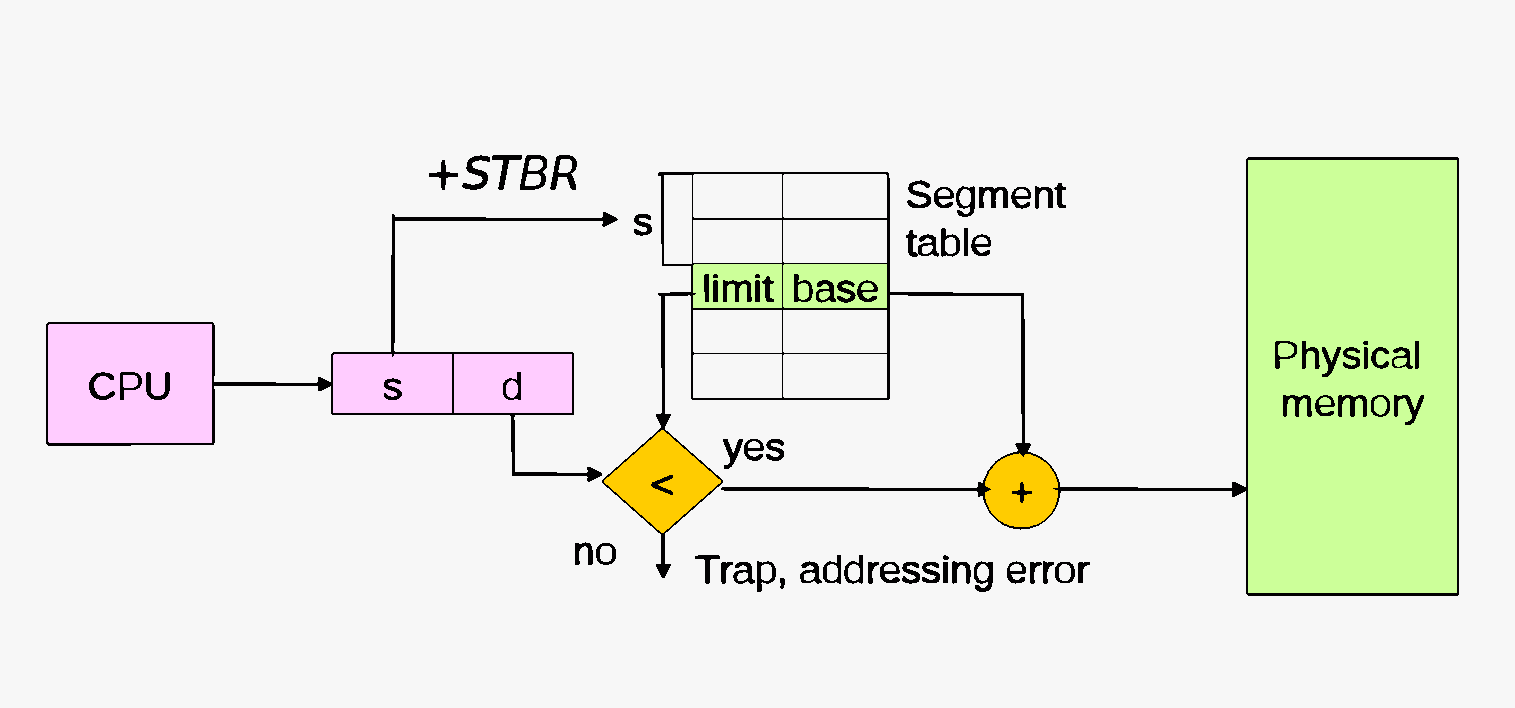
\includegraphics[width=0.90\textwidth]{assets/SegmentationTranslation.pdf}
    \end{center}
    \caption{Traducción de direcciones en un sistema con Segmentación}\label{fig:}
\end{figure}
\pagebreak
\subsubsection{Segmentación Paginada}
\begin{itemize}
    \item La paginación:
    \begin{itemize}
        \item Transparente al programador.
        \item Elimina Fragmentación Externa.
    \end{itemize}
    \item La segmentación:
    \begin{itemize}
        \item Es visible al programador.
        \item Facilita modularidad, estructuras de datos grandes y da mejor soporte a la compartición y protección.
    \end{itemize}
    \item \textbf{Segmentación Paginada:} cada segmento es dividido en páginas de tamaño fijo.
\end{itemize}
\begin{figure}[h]
    \begin{center}
        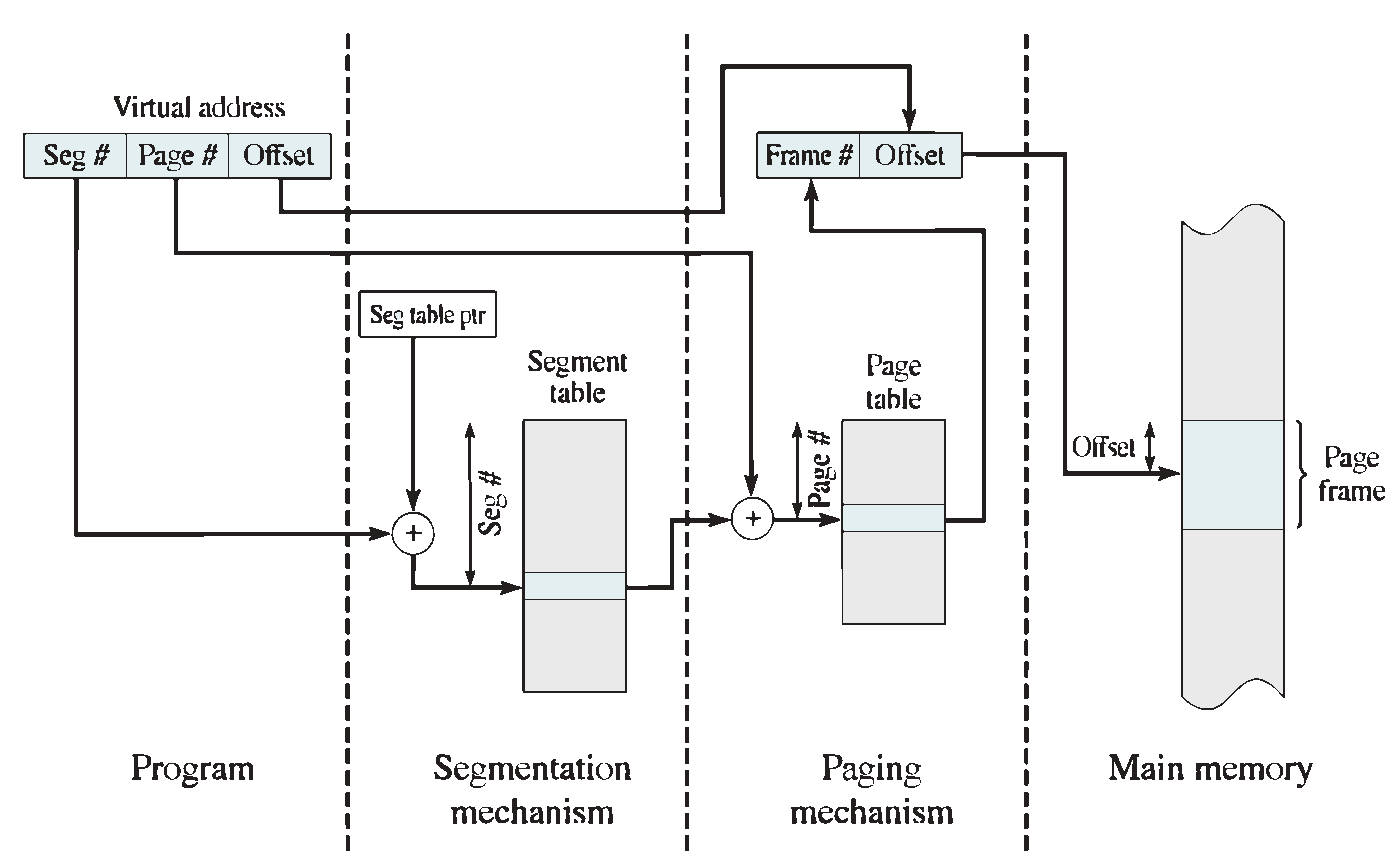
\includegraphics[width=0.95\textwidth]{assets/SegmentacionPaginada.pdf}
    \end{center}
    \caption{Traducción de direcciones en un sistema con Segmentacion Paginada}\label{fig:}
\end{figure}


\end{document}
